%% Apêndices

\begin{apendicesenv}
  %% Cada Capítulo será um apêndice
  \chapter{Questionário da Pesquisa de Mercado}
  \label{apendice:questionario}

  Este apêndice apresenta a transcrição fiel do questionário, desenvolvido na plataforma Google Forms, que foi utilizado para o levantamento de requisitos do sistema ViaBus.

  \vspace{1cm} % Adiciona um espaço vertical

  \noindent\textbf{Título do Formulário:} ViaBus: simplificando a gestão do seu transporte de passageiros (pesquisa de mercado)

  \section*{Perguntas}
  \begin{enumerate}
    \item \textbf{Em qual empresa ou serviço você atua? (Opcional)} \\
          \textit{Campo para resposta curta.}

    \item \textbf{Qual o tamanho da frota de veículos?} \\
          \textit{Marcar apenas uma oval.}
          \begin{itemize}
            \item 1 veículo
            \item 2 a 5 veículos
            \item 6 a 10 veículos
            \item 11 a 20 veículos
            \item Mais de 20 veículos
          \end{itemize}

    \item \textbf{Quantas rotas (trechos) diferentes a empresa opera regularmente?} \\
          \textit{Marcar apenas uma oval.}
          \begin{itemize}
            \item 1 a 2 rotas
            \item 3 a 5 rotas
            \item 6 a 10 rotas
            \item Mais de 10 rotas
            \item Não opero rotas fixas (apenas fretamento)
          \end{itemize}

    \item \textbf{A operação é principalmente:} \\
          \textit{Marcar apenas uma oval.}
          \begin{itemize}
            \item Intermunicipal (dentro do mesmo estado)
            \item Interestadual (entre estados diferentes)
            \item Ambos
          \end{itemize}

    \item \textbf{Como é gerenciada a venda de passagens e a lista de passageiros hoje?} \\
          \textit{Marque todas que se aplicam.}
          \begin{itemize}
            \item Caderno de anotações / Planilha em papel
            \item Planilhas no computador (Excel, Google Sheets)
            \item Mensagens diretas (WhatsApp, Telegram)
            \item Ligação telefônica
            \item Diretamente com o motorista, na hora do embarque
            \item Utilizo outro sistema/software
            \item Outro
          \end{itemize}

    \item \textbf{Quais são os maiores desafios operacionais hoje para a empresa?} \\
          \textit{Marque todas que se aplicam.}
          \begin{itemize}
            \item Realizar o embarque de passageiros com planilhas manuais.
            \item Controlar quais assentos já foram vendidos e quais estão livres.
            \item Perda de tempo organizando listas de passageiros e viagens.
            \item Prejuízo com assentos vazios (baixa ocupação)
            \item Comunicação com os motoristas sobre a rota e os passageiros.
            \item Receber os pagamentos (muito dinheiro em espécie, dificuldade com Pix, etc.).
            \item Outro
          \end{itemize}

    \item \textbf{Quão valioso seria ter um sistema único para gerenciar rotas, horários, veículos, motoristas e passagens em um só lugar, acessível pelo celular ou computador?} \\
          \textit{Marcar apenas uma oval, em uma escala de 1 a 5.}
          \begin{itemize}
            \item 1 \quad 2 \quad 3 \quad 4 \quad 5
          \end{itemize}

    \item \textbf{Quais funcionalidades de um sistema como o ViaBus seriam mais importantes para o seu negócio?} \\
          \textit{Marque todas que se aplicam.}
          \begin{itemize}
            \item Embarque facilitado através de um aplicativo/site, substituindo planilhas manuais.
            \item Painel para cadastrar e organizar minhas rotas, horários e preços.
            \item Possibilidade de agendamento externo (ex.: prefeituras às quais a empresa presta serviços).
            \item Venda de passagens online (com pagamento por Pix e cartão).
            \item Cadastro e gestão de motoristas e veículos.
            \item Relatórios financeiros (vendas por período, por rota, etc.).
            \item Outro
          \end{itemize}

    \item \textbf{Se você pudesse oferecer aos seus passageiros um aplicativo para eles mesmos comprarem e acompanharem a viagem (ver horário, paradas, etc.), você acredita que isso seria um diferencial contra seus concorrentes?} \\
          \textit{Marcar apenas uma oval.}
          \begin{itemize}
            \item Sim, com certeza seria um grande diferencial.
            \item Talvez, poderia atrair mais clientes.
            \item Não, acho que não faria diferença.
            \item Tenho dúvidas se meus clientes usariam.
          \end{itemize}

    \item \textbf{Qual modelo de parceria você consideraria mais justo para usar um sistema completo como este?} \\
          \textit{Marcar apenas uma oval.}
          \begin{itemize}
            \item Uma pequena taxa fixa por mês.
            \item Uma pequena porcentagem (\%) sobre cada passagem vendida pelo sistema.
            \item Um modelo misto (taxa mensal baixa + porcentagem pequena).
            \item Não tenho certeza.
          \end{itemize}

    \item \textbf{Gostaria de receber um convite para testar a plataforma ViaBus em primeira mão e sem custos quando estiver disponível?} \\
          \textit{Marcar apenas uma oval.}
          \begin{itemize}
            \item Sim, tenho interesse!
            \item Não, obrigado.
            \item Talvez, gostaria de mais informações antes.
          \end{itemize}
  \end{enumerate}


  \chapter{Resultados da Pesquisa de Mercado}
  \label{apendice:resultados}

  Este apêndice apresenta os resultados visuais coletados através da pesquisa de mercado realizada com dois gestores de empresas de transporte de passageiros.

  \begin{figure}[htbp]
    \centering
    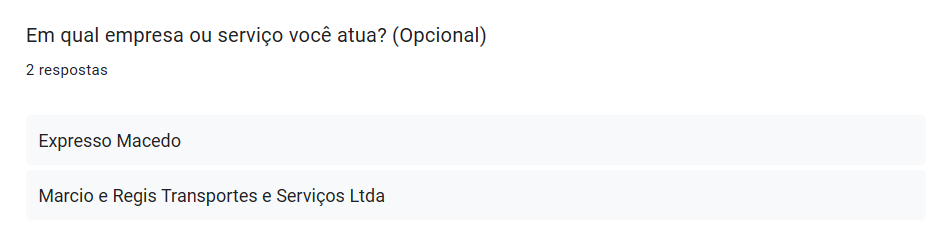
\includegraphics[width=0.8\textwidth]{imagens/imagem1.png}
    \caption{Resultado da pergunta sobre empresa ou serviço.}
    \label{fig:resultado1}
  \end{figure}

  \begin{figure}[htbp]
    \centering
    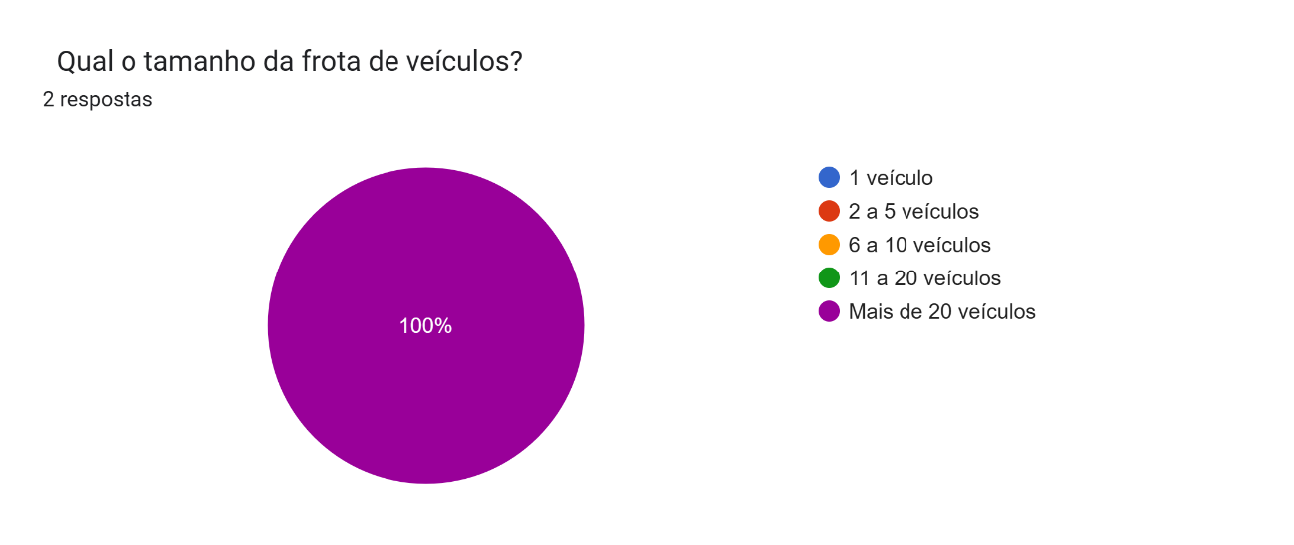
\includegraphics[width=0.8\textwidth]{imagens/imagem2.png}
    \caption{Resultado da pergunta sobre tamanho da frota de veículos.}
    \label{fig:resultado2}
  \end{figure}

  \begin{figure}[htbp]
    \centering
    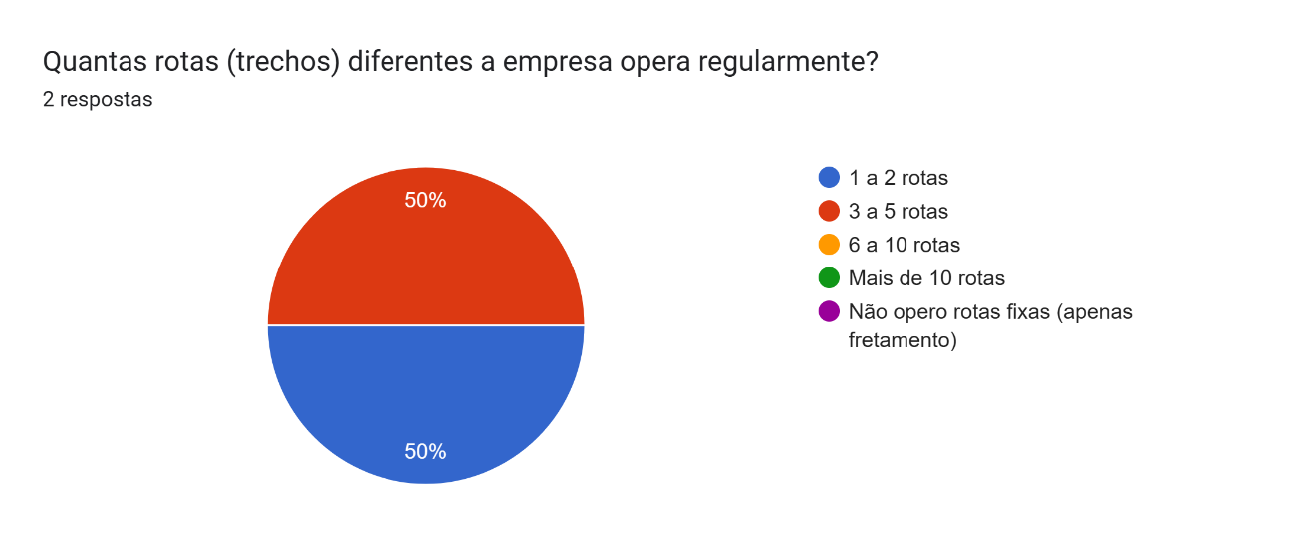
\includegraphics[width=0.8\textwidth]{imagens/imagem3.png}
    \caption{Resultado da pergunta sobre número de rotas operadas.}
    \label{fig:resultado3}
  \end{figure}

  \begin{figure}[htbp]
    \centering
    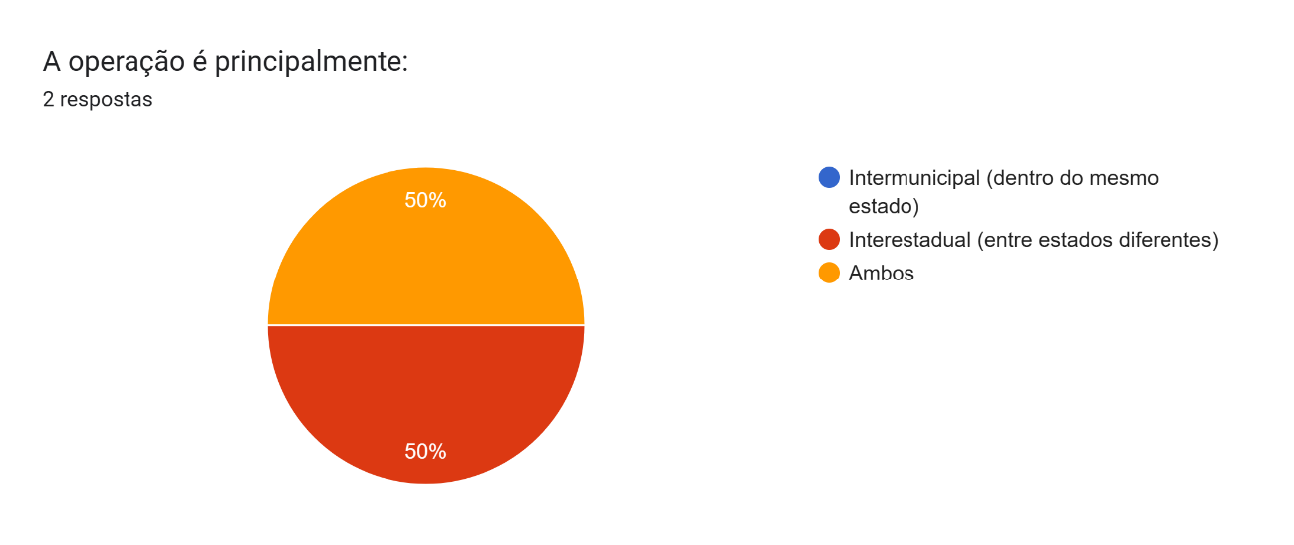
\includegraphics[width=0.8\textwidth]{imagens/imagem4.png}
    \caption{Resultado da pergunta sobre tipo de operação.}
    \label{fig:resultado4}
  \end{figure}

  \begin{figure}[htbp]
    \centering
    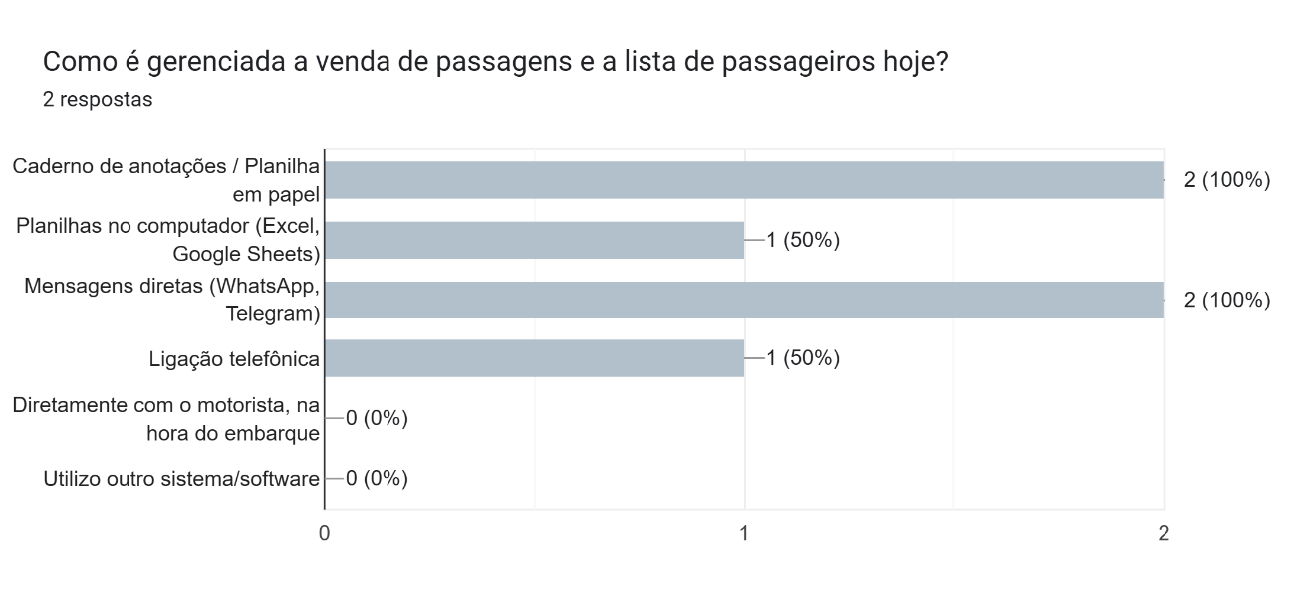
\includegraphics[width=0.8\textwidth]{imagens/imagem5.png}
    \caption{Resultado da pergunta sobre gerenciamento atual de passagens.}
    \label{fig:resultado5}
  \end{figure}

  \begin{figure}[htbp]
    \centering
    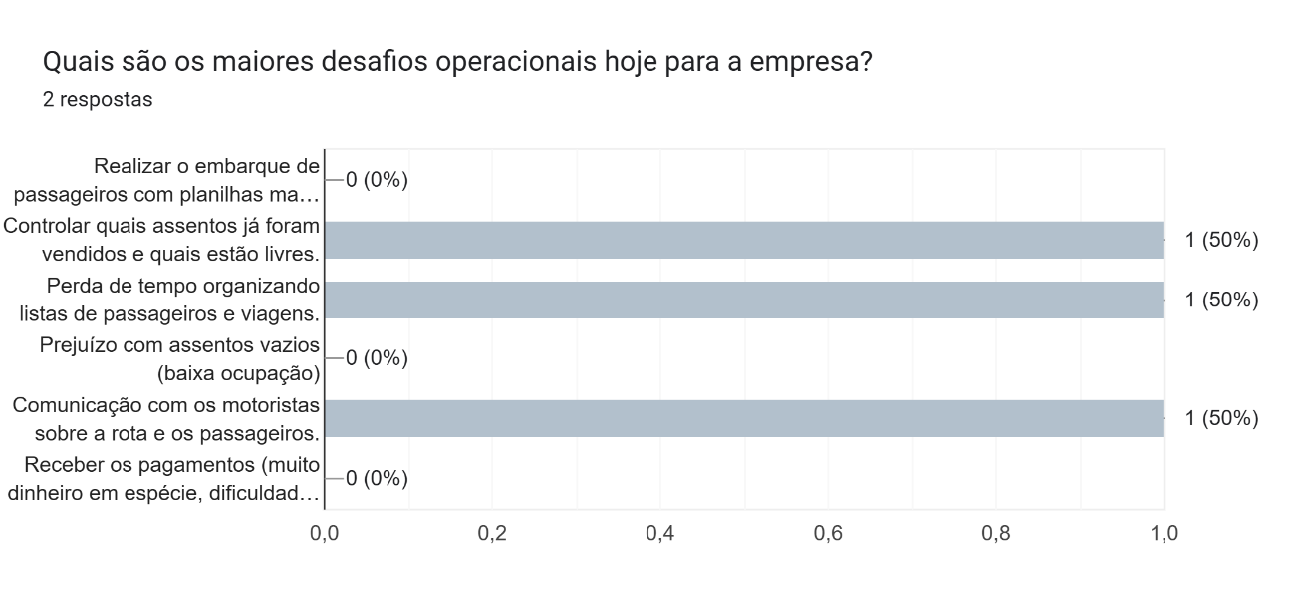
\includegraphics[width=0.8\textwidth]{imagens/imagem6.png}
    \caption{Resultado da pergunta sobre maiores desafios operacionais.}
    \label{fig:resultado6}
  \end{figure}

  \begin{figure}[htbp]
    \centering
    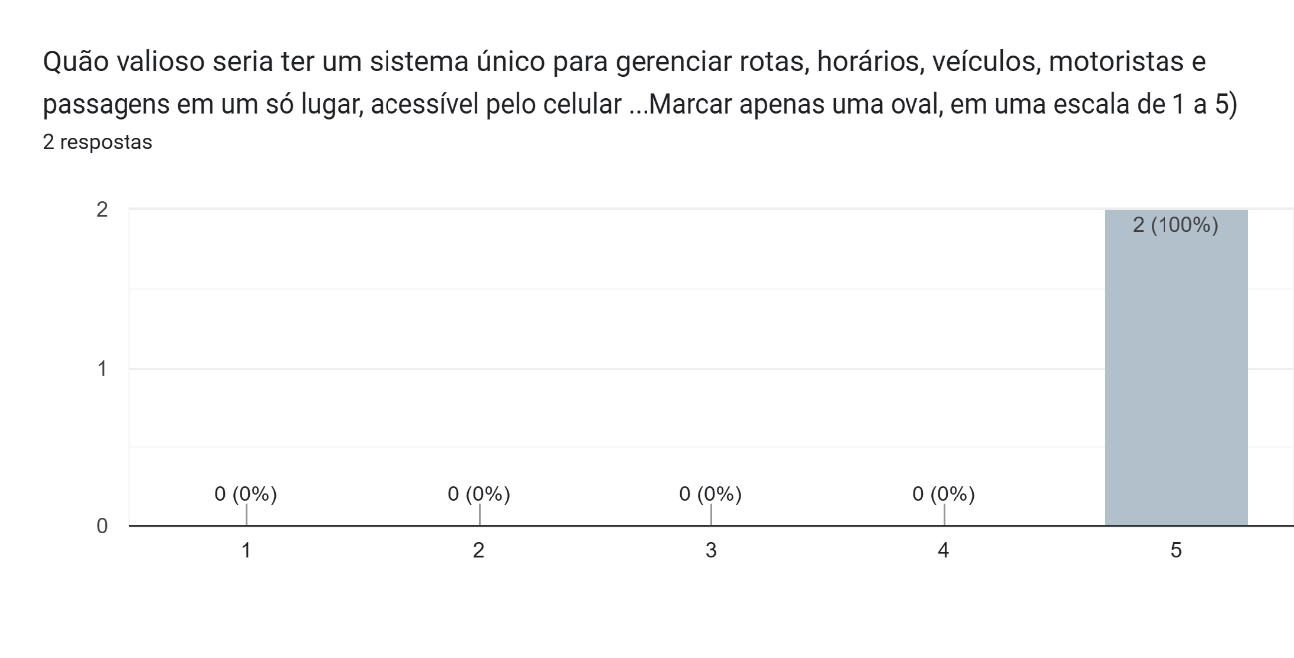
\includegraphics[width=0.8\textwidth]{imagens/imagem7.png}
    \caption{Resultado da pergunta sobre valor de um sistema único.}
    \label{fig:resultado7}
  \end{figure}

  \begin{figure}[htbp]
    \centering
    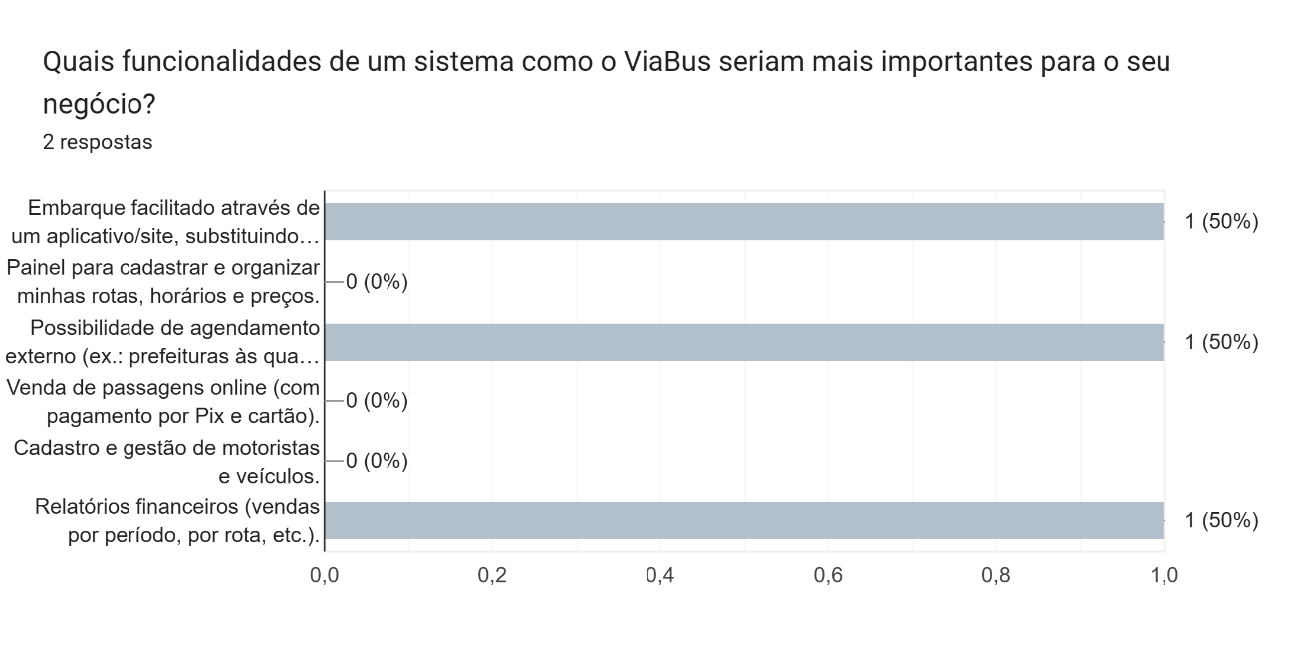
\includegraphics[width=0.8\textwidth]{imagens/imagem8.png}
    \caption{Resultado da pergunta sobre funcionalidades mais importantes.}
    \label{fig:resultado8}
  \end{figure}

  \begin{figure}[htbp]
    \centering
    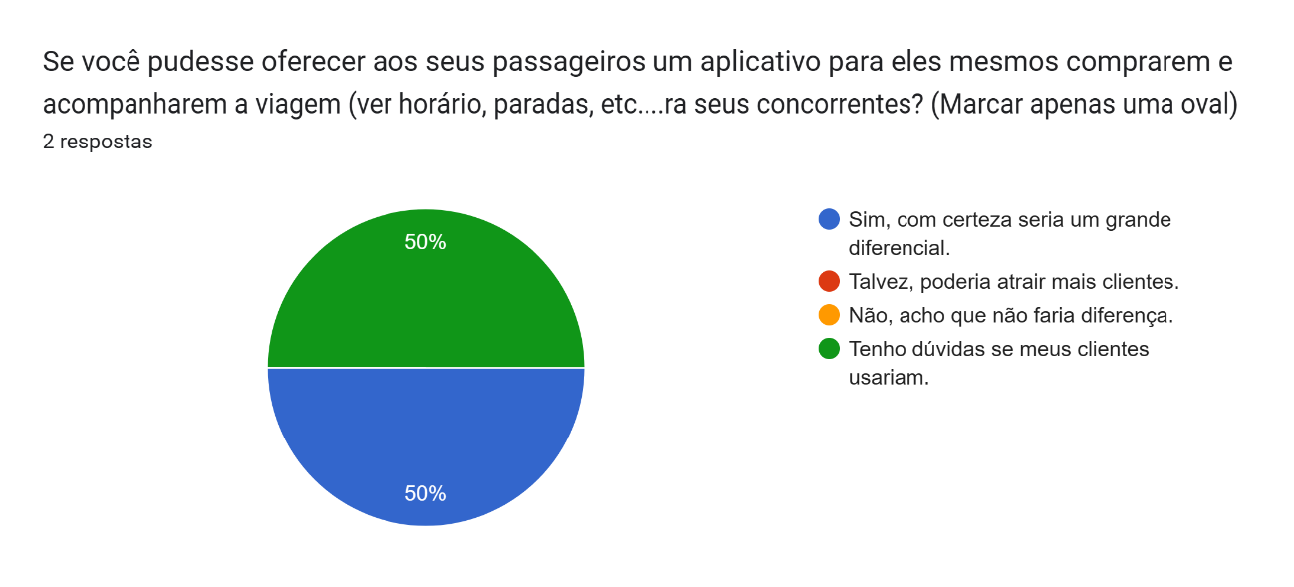
\includegraphics[width=0.8\textwidth]{imagens/imagem9.png}
    \caption{Resultado da pergunta sobre aplicativo como diferencial.}
    \label{fig:resultado9}
  \end{figure}

  \begin{figure}[htbp]
    \centering
    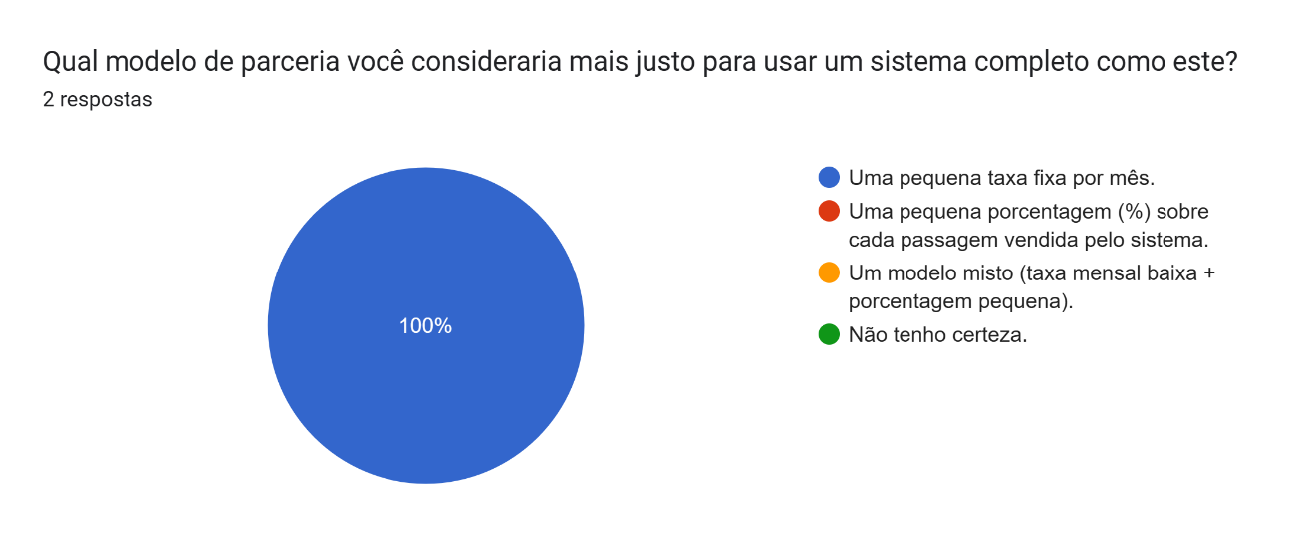
\includegraphics[width=0.8\textwidth]{imagens/imagem10.png}
    \caption{Resultado da pergunta sobre modelo de parceria.}
    \label{fig:resultado10}
  \end{figure}

  \begin{figure}[htbp]
    \centering
    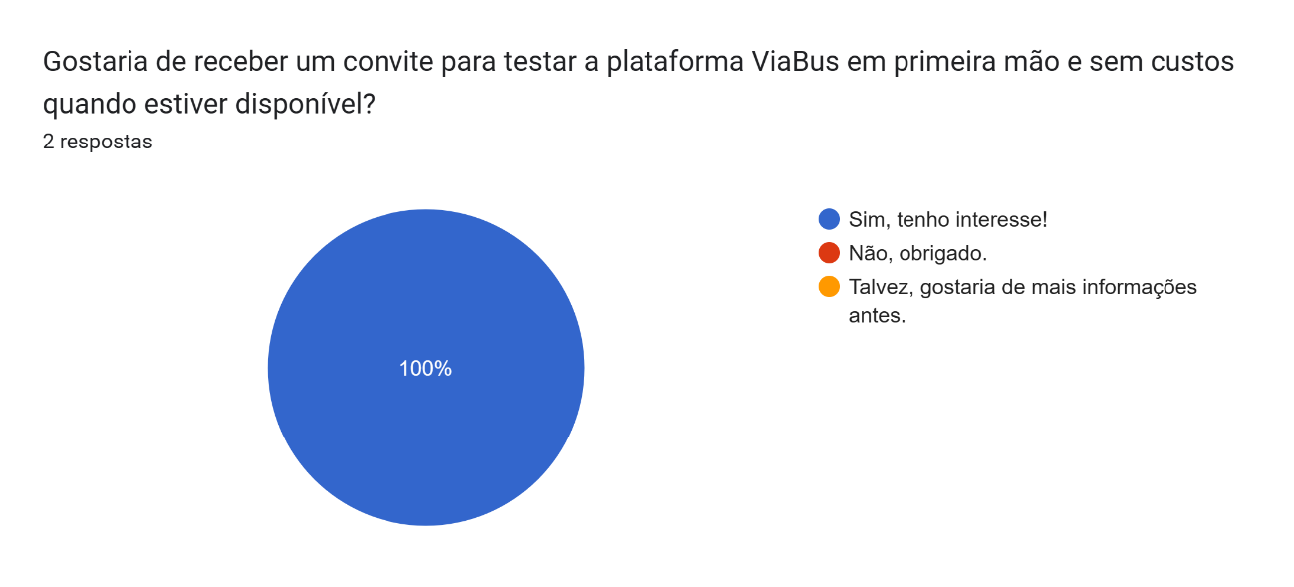
\includegraphics[width=0.8\textwidth]{imagens/imagem11.png}
    \caption{Resultado da pergunta sobre interesse em testar a plataforma.}
    \label{fig:resultado11}
  \end{figure}

  \chapter{Diagrama de Classe do ViaBus}
  \label{apendice:diagrama-classe}

  \begin{figure}[H]
    \centering
    \begin{tikzpicture}[scale=0.4, every node/.style={transform shape}]
      \tikzumlset{font=\tiny}

      % NÍVEL 1: Empresa (topo da hierarquia)
      \umlclass[x=18,y=25]{Company}{
        id: uuid\\
        legalName: string\\
        tradeName: string\\
        slug: string\\
        cnpj: string\\
        email: string\\
        phone: string\\
        logoUrl: string\\
        createdAt: Date\\
        updatedAt: Date
      }{ }

      % NÍVEL 2: Gestão de usuários e recursos
      \umlclass[x=3,y=18]{User}{
        id: uuid\\
        name: string\\
        email: string\\
        phone: string\\
        photoUrl: string\\
        password: string\\
        role: UserRole\\
        status: UserStatus\\
        companyId: uuid\\
        createdAt: Date\\
        updatedAt: Date
      }{ }

      \umlclass[x=18,y=18]{Vehicle}{
        id: uuid\\
        plate: string\\
        model: string\\
        brand: string\\
        year: number\\
        capacity: number\\
        category: VehicleCategory\\
        comfortConfiguration: ComfortConfiguration\\
        busType: BusType\\
        acquisitionDate: Date\\
        odometer: number\\
        lastMaintenance: Date\\
        nextMaintenance: Date\\
        status: VehicleStatus\\
        notes: string\\
        companyId: uuid
      }{ }

      \umlclass[x=33,y=18]{Driver}{
        id: uuid\\
        name: string\\
        cpf: string\\
        licenseNumber: string\\
        licenseCategory: string\\
        licenseExpiry: Date\\
        phone: string\\
        email: string\\
        birthDate: Date\\
        hireDate: Date\\
        status: DriverStatus\\
        emergencyContactName: string\\
        emergencyContactPhone: string\\
        address: string\\
        notes: string\\
        companyId: uuid
      }{ }

      % NÍVEL 3: Configuração de rotas
      \umlclass[x=8,y=11]{Route}{
        id: uuid\\
        name: string\\
        description: string\\
        isActive: boolean\\
        estimatedDuration: string\\
        distance: number\\
        companyId: uuid
      }{ }

      \umlclass[x=23,y=11]{Stop}{
        id: uuid\\
        name: string\\
        addressId: uuid\\
        isActive: boolean\\
        hasAccessibility: boolean\\
        hasShelter: boolean\\
        companyId: uuid
      }{ }

      \umlclass[x=38,y=11]{Address}{
        id: uuid\\
        cep: string\\
        street: string\\
        number: string\\
        complement: string\\
        neighborhood: string\\
        city: string\\
        state: string\\
        longitude: number\\
        latitude: number\\
        createdAt: Date\\
        updatedAt: Date
      }{ }

      % NÍVEL 4: Relacionamentos de configuração
      \umlclass[x=8,y=4]{RouteSchedule}{
        id: uuid\\
        routeId: uuid\\
        dayOfWeek: number\\
        isActive: boolean\\
        createdAt: Date\\
        updatedAt: Date
      }{ }

      \umlclass[x=23,y=4]{RouteStop}{
        id: uuid\\
        routeId: uuid\\
        stopId: uuid\\
        order: number\\
        departureTime: string
      }{ }

      % NÍVEL 5: Operação - Viagens
      \umlclass[x=3,y=-3]{TripVehicle}{
        id: uuid\\
        tripId: uuid\\
        vehicleId: uuid\\
        primaryDriverId: uuid\\
        secondaryDriverId: uuid\\
        isActive: boolean\\
        observations: string\\
        createdAt: Date\\
        updatedAt: Date
      }{ }

      \umlclass[x=18,y=-3]{Trip}{
        id: uuid\\
        routeId: uuid\\
        departureTime: Date\\
        estimatedArrivalTime: Date\\
        actualDepartureTime: Date\\
        actualArrivalTime: Date\\
        status: TripStatus\\
        basePrice: number\\
        totalSeats: number\\
        availableSeats: number\\
        isAutoGenerated: boolean\\
        observations: string\\
        companyId: uuid\\
        createdAt: Date\\
        updatedAt: Date
      }{ }

      % NÍVEL 6: Vendas - Bilhetes
      \umlclass[x=33,y=-3]{Ticket}{
        id: uuid\\
        tripId: uuid\\
        passengerName: string\\
        passengerDocument: string\\
        passengerPhone: string\\
        passengerEmail: string\\
        seatNumber: string\\
        price: number\\
        status: TicketStatus\\
        boardingPointType: BoardingPointType\\
        boardingStopId: uuid\\
        boardingLocationDescription: string\\
        boardingLatitude: number\\
        boardingLongitude: number\\
        landingPointType: BoardingPointType\\
        landingStopId: uuid\\
        landingLocationDescription: string\\
        landingLatitude: number\\
        landingLongitude: number\\
        observations: string\\
        companyId: uuid
      }{ }

      % RELACIONAMENTOS HIERÁRQUICOS PRINCIPAIS
      % Company -> Recursos
      \umlassoc[mult1=1,mult2=*]{Company}{User}
      \umlassoc[mult1=1,mult2=*]{Company}{Vehicle}
      \umlassoc[mult1=1,mult2=*]{Company}{Driver}

      % Company -> Configuração
      \umlassoc[mult1=1,mult2=*,arm1=-135,arm2=90]{Company}{Route}
      \umlassoc[mult1=1,mult2=*,arm1=-45,arm2=90]{Company}{Stop}

      % Configuração de endereços
      \umlassoc[mult1=1,mult2=*]{Address}{Stop}

      % FLUXO PRINCIPAL: Route -> RouteStop <- Stop
      \umlassoc[mult1=1,mult2=*]{Route}{RouteStop}
      \umlassoc[mult1=1,mult2=*]{Stop}{RouteStop}

      % Horários das rotas
      \umlassoc[mult1=1,mult2=*]{Route}{RouteSchedule}

      % FLUXO OPERACIONAL: Route -> Trip
      \umlassoc[mult1=1,mult2=*]{Route}{Trip}
      \umlassoc[mult1=1,mult2=*,arm1=-135,arm2=90]{Company}{Trip}

      % Trip -> TripVehicle (associação veículo/motorista)
      \umlassoc[mult1=1,mult2=*]{Trip}{TripVehicle}
      \umlassoc[mult1=1,mult2=*,arm1=-90,arm2=90]{Vehicle}{TripVehicle}
      \umlassoc[mult1=1,mult2=*,arm1=-90,arm2=135,stereo=<<primaryDriver>>]{Driver}{TripVehicle}

      % FLUXO DE VENDAS: Trip -> Ticket
      \umlassoc[mult1=1,mult2=*]{Trip}{Ticket}
      \umlassoc[mult1=1,mult2=*,arm1=-45,arm2=135]{Company}{Ticket}

      % Relacionamento opcional: Stop -> Ticket (embarque/desembarque específico)
      \umldep[stereo=<<boarding/landing>>,mult1=0..1,mult2=*,arm1=-90,arm2=135]{Stop}{Ticket}

    \end{tikzpicture}
    \caption{Diagrama de classes detalhado do domínio ViaBus.}
    \label{fig:uml-dominio}
  \end{figure}

  \chapter{Repositórios do Código-Fonte}
  \label{apendice:repositorios}

  O código-fonte completo do protótipo do sistema ViaBus, desenvolvido como parte deste trabalho, está publicamente disponível para consulta e análise nos seguintes repositórios da plataforma GitHub:

  \vspace{1cm}

  \begin{itemize}
    \item \textbf{Repositório do Frontend (Interface do Usuário):} \\
          \url{https://github.com/JeanCarlos899/viabus-front-end}

    \item \textbf{Repositório do Backend (API e Lógica de Negócio):} \\
          \url{https://github.com/JeanCarlos899/viabus-back-end}
  \end{itemize}
\end{apendicesenv}